\documentclass{beamer}
\usetheme{Singapore}
\usecolortheme{beaver}
\usepackage{subfig}
\usepackage{braket}



\title{Quantum Communication Complexity}
\author{James Hawley}
\date{August 15, 2014}
\institute{Institute for Quantum Computing\\University of Waterloo}
\graphicspath{{./img/}}


\begin{document}

\begin{frame}
\titlepage
\end{frame}

\section*{Contents}
\begin{frame}{Contents}
\tableofcontents
\end{frame}

\section{Background}
\subsection{Quantum Computing}

%\begin{frame}{Communication Complexity}
%\begin{center}
%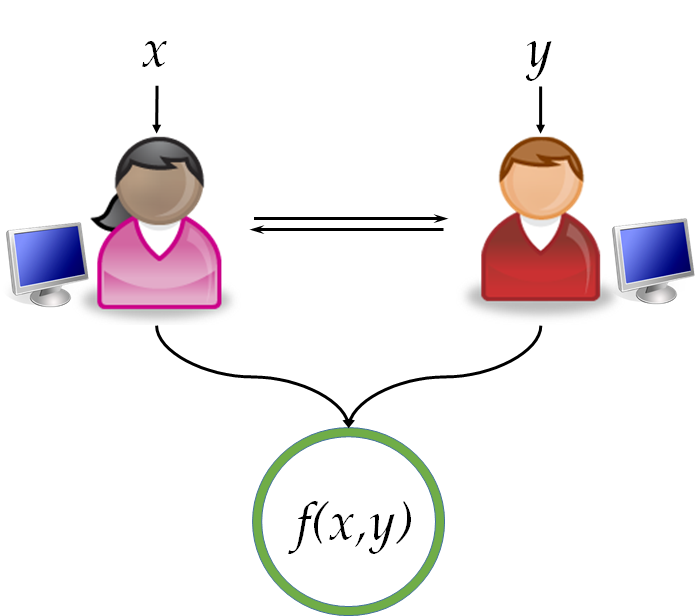
\includegraphics[width=0.5\textwidth]{twoway_communication.png}
%\end{center}
%\begin{itemize}
%\item<2-> Measure information exchanged
%\item<3-> Find and develop algorithms
%\end{itemize}
%\end{frame}

%\begin{frame}{Communication Complexity}
%\begin{figure}[!h]
%\subfloat[One-way communication]{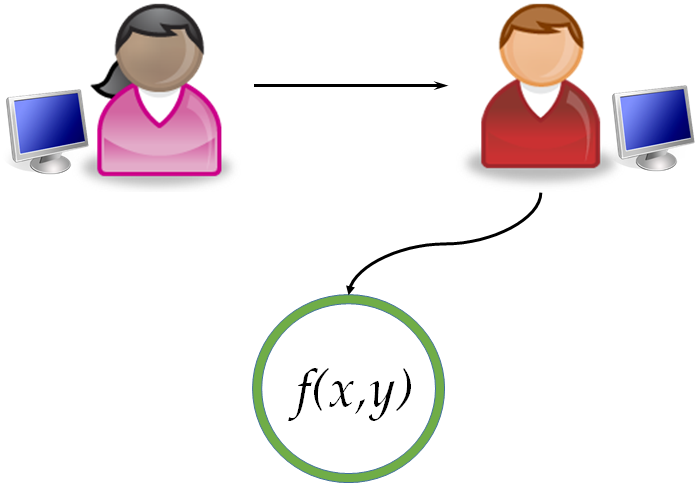
\includegraphics[width=0.5\textwidth]{oneway_communication.png}}
%\subfloat[Refereed communication]{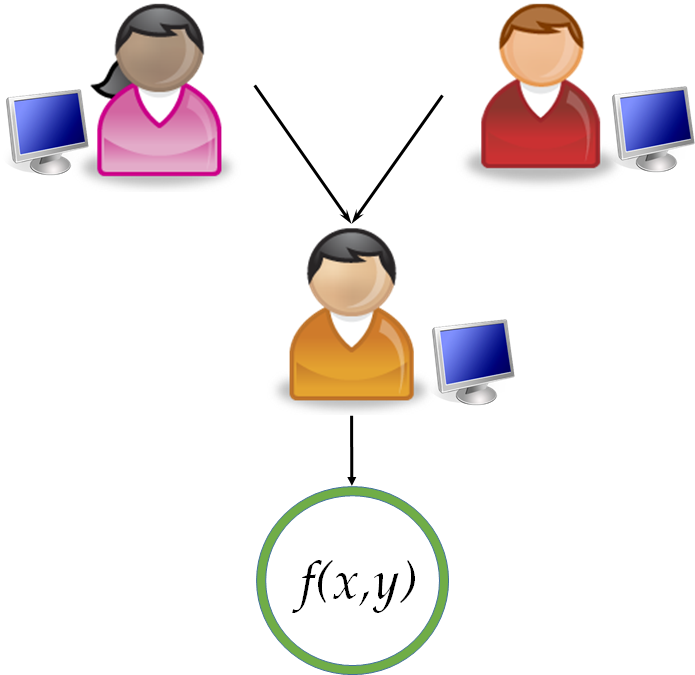
\includegraphics[width=0.5\textwidth]{no_communication.png}}
%\end{figure}
%\end{frame}

\begin{frame}{Qubit/Qudit Model}
\begin{itemize}
\item<2-> Qubit: $\ket{\psi} = \alpha\ket{0} + \beta\ket{1}$
\item<3-> Qudit: $\ket{\psi} = \sum\limits_{k=0}^{d-1}\alpha_k \ket{k}$
\item<4-> Logic gates $\rightarrow$ unitary operators
\end{itemize}
\end{frame}

\subsection{Stabilizers and the Discrete Wigner Function}
\begin{frame}{Stabilizers}
\begin{itemize}
\item<2-> Weyl-Heisenberg Operators
\begin{center}
$D_d = \{e^{\frac{i\pi x z}{d}}Z^zX^x | x,z \in \mathbb{Z}_d\}$\\
$Z = \left( \begin{array}{cccc}
	1 & &  & \\
	 & e^{\frac{i2\pi}{d}} &  & \\
	 & & \ddots & \\
	 & & & e^{\frac{i2\pi}{d}(d-1)}\\
	\end{array} \right)$
$X = \left( \begin{array}{cccc}
	 & & & 1\\
	1 & & 0 &\\
	 & \ddots & &\\
	0 & & 1 &\\
	\end{array} \right)$
\end{center}
\item<3-> Clifford Unitary Operators
\begin{center}
$C_{d,n} = \{U\in\mathcal{U}(d^n) | U \mathcal{h}D_d^{\otimes n}\mathcal{i} U^\dag = \mathcal{h}D_d^{\otimes n}\mathcal{i}\}$
\end{center}
\item<4-> Gottesman-Knill Theorem
\end{itemize}
\end{frame}

\begin{frame}{Discrete Wigner Function}
\begin{itemize}
\item<2-> Representation in discrete phase space
\item<3-> $W_\rho(\alpha) = \frac{1}{d}$Tr$(\rho A_\alpha)$
\item<3-> Stabilizers $\implies W_\rho(\alpha) \ge 0 \forall \alpha \in \mathbb{Z}_d^2$
\item<4->$W_U(\beta | \alpha) = \frac{1}{d}$Tr$(A_\beta U A_\alpha U^\dag)$
\item<4->Clifford $\implies W_U(\beta | \alpha) \ge 0 \forall \alpha,\beta \in \mathbb{Z}_d^2$
\item<5-> $\mathcal{M}_\rho = \sum\limits_{\alpha \in \mathbb{Z}_d^2} |W_\rho(\alpha)|$
\item<5-> $\mathcal{M}_U = \max\limits_{\alpha \in \mathbb{Z}_d^2} \sum\limits_{\beta \in \mathbb{Z}_d^2} |W_U(\beta | \alpha)|$
\end{itemize}
\end{frame}

\section{Main Work}
\subsection{Raz's Problem}
\begin{frame}{Raz's Problems}
\begin{center}
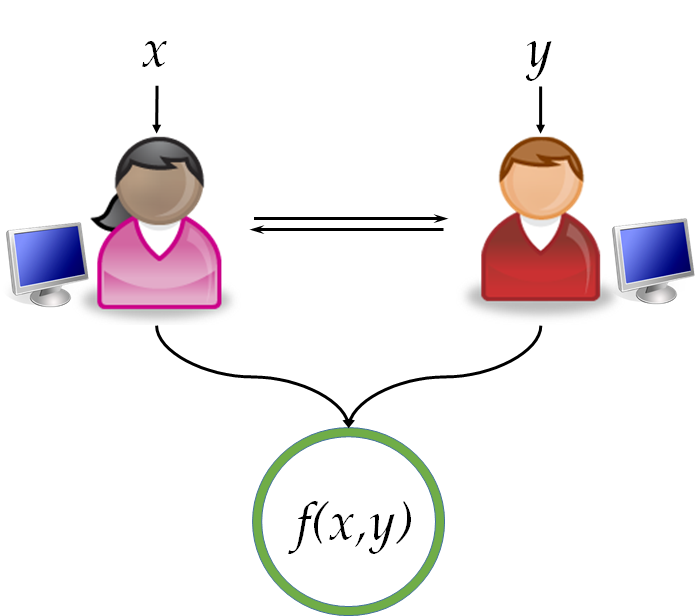
\includegraphics[width=0.5\textwidth]{twoway_communication.png}
\end{center}
\begin{itemize}
\item<2-> Measure information exchanged
\item<3-> Early proof of exponential separation
\item<4-> Two main variants
\item<5-> $O($log$d)$ communication complexity for quantum algorithm
\end{itemize}
\end{frame}

\begin{frame}{Raz's Problem: Variant 1}
\begin{figure}[!h]
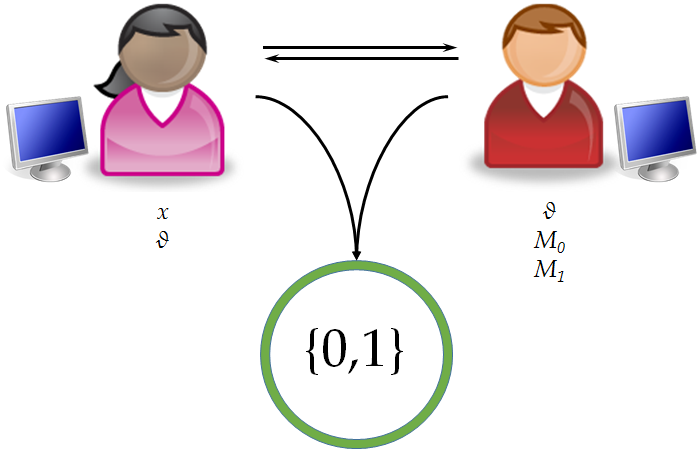
\includegraphics[width=0.7\textwidth]{Raz_prob1.png}
\end{figure}
\begin{itemize}
\item Return 0 if d$(x, M_0) < \vartheta$, 1 otherwise
\end{itemize}
\end{frame}

\begin{frame}{Raz's Problem: Variant 2}
\begin{figure}[!h]
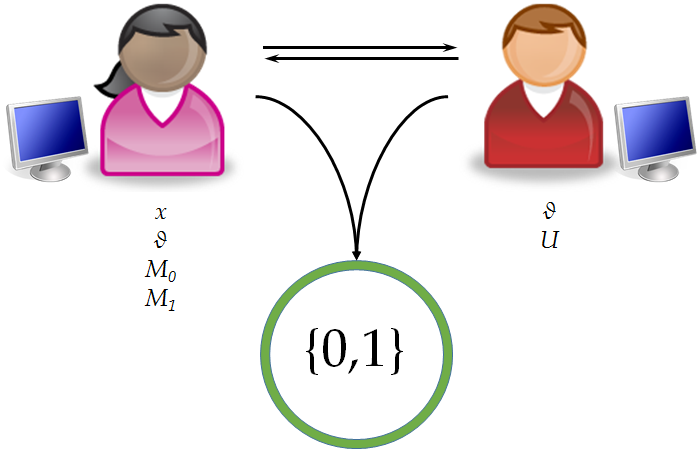
\includegraphics[width=0.7\textwidth]{Raz_prob2.png}
\end{figure}
\begin{itemize}
\item Return 0 if d$(Ux, M_0) < \vartheta$, 1 otherwise
\end{itemize}
\end{frame}

\subsection{Solutions}
\begin{frame}{Convergence and Complexity}
\begin{itemize}
\item<2-> Stabilizers $\implies O($log$d)$ complexity
\item<3-> At most $O(d^3$log$d)$ complexity
\item<4-> $\text{Pr}(|\hat{R} - \mathbb{E}(R)|) \ge \epsilon) \le 2e^{\frac{-T\epsilon^2}{2\mathcal{M}^2}}$
\end{itemize}
\end{frame}

\section{Acknowledgments and References}
\begin{frame}{Acknowlegments}
\begin{itemize}
\item Joseph Emerson
\item Joel Wallman
\item Mark Howard
\end{itemize}
\end{frame}

\begin{frame}{Refrences}
\begin{enumerate}
\item Hakop Pashayan, Joel J Wallman, and Stephen D Bartlett. “Simulating quantum circuits with
quasiprobabilities”. 2014.
\item Ran Raz. “Exponential separation of quantum and classical communication complexity”. Pro-
ceedings of the 31st Annual ACM Symposium on Theory of Computing (1999), pp. 358–367.
doi : 10.1145/301250.301343.
\item Michael M Wolf. “Quantum Channels \& Operations Guided Tour”. Copenhagen, 2012.
\item William K. Wootters. “A Wigner-Function Formulation of Quantum Mechanics”. Annals of
Physics 176 (1987), pp. 1–21. doi : 10.1016/0003-4916(87)90176-X.
\end{enumerate}
\end{frame}

\end{document}